\documentclass[border=4pt]{standalone}

\usepackage{amsmath}
\usepackage{tikz}
\usepackage{mathdots}
\usepackage{yhmath}
\usepackage{cancel}
\usepackage{color}
\usepackage{siunitx}
\usepackage{array}
\usepackage{multirow}
\usepackage{amssymb}
\usepackage{gensymb}
\usepackage{tabularx}
\usepackage{booktabs}
\usetikzlibrary{fadings}
\usetikzlibrary{patterns}


\begin{document}
 
 


\tikzset{every picture/.style={line width=0.75pt}} %set default line width to 0.75pt        

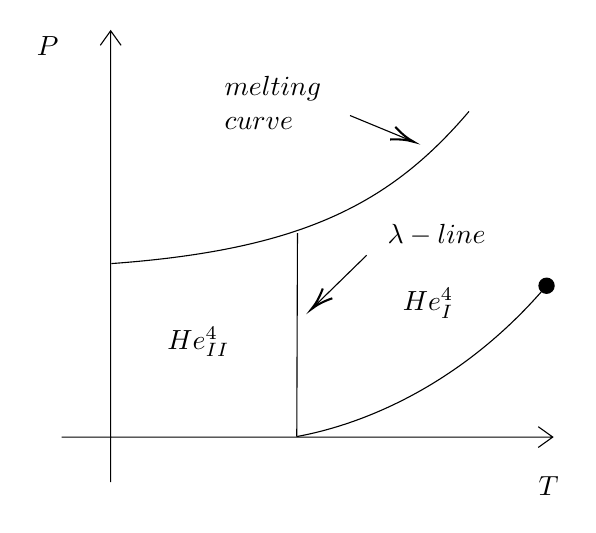
\begin{tikzpicture}[x=0.75pt,y=0.75pt,yscale=-1,xscale=1]
%uncomment if require: \path (0,457); %set diagram left start at 0, and has height of 457

%Shape: Axis 2D [id:dp25715428677652574] 
\draw  (186,265.92) -- (422.67,265.92)(209.67,70.17) -- (209.67,287.67) (415.67,260.92) -- (422.67,265.92) -- (415.67,270.92) (204.67,77.17) -- (209.67,70.17) -- (214.67,77.17)  ;
%Curve Lines [id:da5161002642571322] 
\draw    (210,182.33) .. controls (301.67,175.67) and (344.33,153.67) .. (382.33,109) ;


%Curve Lines [id:da956281140078328] 
\draw    (299.33,265.67) .. controls (335.67,259) and (381.67,237.67) .. (419.67,193) ;


%Straight Lines [id:da36671347094422724] 
\draw    (299.67,167.67) -- (299.33,265.67) ;


%Straight Lines [id:da8984665547038162] 
\draw    (333,178.33) -- (307.77,202.94) ;
\draw [shift={(306.33,204.33)}, rotate = 315.73] [color={rgb, 255:red, 0; green, 0; blue, 0 }  ][line width=0.75]    (10.93,-3.29) .. controls (6.95,-1.4) and (3.31,-0.3) .. (0,0) .. controls (3.31,0.3) and (6.95,1.4) .. (10.93,3.29)   ;

%Straight Lines [id:da38580231689935207] 
\draw    (325,111) -- (353.82,122.9) ;
\draw [shift={(355.67,123.67)}, rotate = 202.44] [color={rgb, 255:red, 0; green, 0; blue, 0 }  ][line width=0.75]    (10.93,-3.29) .. controls (6.95,-1.4) and (3.31,-0.3) .. (0,0) .. controls (3.31,0.3) and (6.95,1.4) .. (10.93,3.29)   ;

%Shape: Circle [id:dp7808714535477603] 
\draw  [fill={rgb, 255:red, 0; green, 0; blue, 0 }  ,fill opacity=1 ] (416,193) .. controls (416,190.97) and (417.64,189.33) .. (419.67,189.33) .. controls (421.69,189.33) and (423.33,190.97) .. (423.33,193) .. controls (423.33,195.03) and (421.69,196.67) .. (419.67,196.67) .. controls (417.64,196.67) and (416,195.03) .. (416,193) -- cycle ;

% Text Node
\draw (420.67,289.33) node   {$T$};
% Text Node
\draw (179.33,77.67) node   {$P$};
% Text Node
\draw (252,220) node   {$He^{4}_{II}$};
% Text Node
\draw (362.67,201.33) node   {$He^{4}_{I}$};
% Text Node
\draw (366.67,168.67) node   {$\lambda -line$};
% Text Node
\draw (290,106.33) node   {$ \begin{array}{l}
melting\ \\
curve
\end{array}$};


\end{tikzpicture}

\end{document}
